\section{Modifying and applying Grad-CAM}
\nblink{brats/07\_gradcam.ipynb}

The basic idea how to apply interpretability methods built for classification on image segmentation tasks is quite simple: The output of a classification model
is a list of confidence scores, one for every class the model can detect. In a segmentation task, the output is a list of pixels with an intensity value.
What we can do is interpret every output pixel as if was a separate class in a classification task.
In a classification task, we are only interested in the highest class value. In a segmentation task, we are interested why a specific pixel from the ground truth did
or did not show up in the network output.

As a first step, we can analyze a saliency map generated for a single class. In the following Result chapter, we analyze the pixel indicated by a red dot.

\subsection{Results}

\begin{figure}[H]
    \centering
    \begin{subfigure}{.33\textwidth}
        \centering
        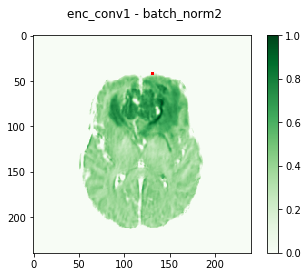
\includegraphics[width=\linewidth]{chapters/04_segmentation/images/grad_cam_03.png}
        \caption{First batch norm layer of the first encoder block}
    \end{subfigure}%
    \begin{subfigure}{.33\textwidth}
        \centering
        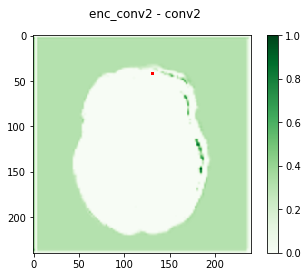
\includegraphics[width=\linewidth]{chapters/04_segmentation/images/grad_cam_05.png}
        \caption{Second convolutional layer in the second encoder block}
    \end{subfigure}%
        \begin{subfigure}{.33\textwidth}
        \centering
        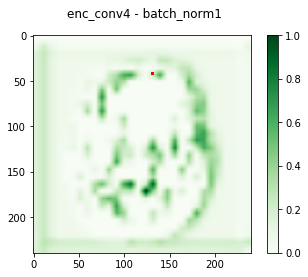
\includegraphics[width=\linewidth]{chapters/04_segmentation/images/grad_cam_14.png}
        \caption{First batch norm layer of the first encoder block}
    \end{subfigure}

    \begin{subfigure}{.33\textwidth}
        \centering
        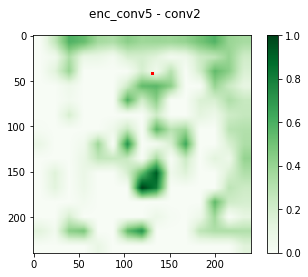
\includegraphics[width=\linewidth]{chapters/04_segmentation/images/grad_cam_17.png}
        \caption{First batch norm layer of the first encoder block}
    \end{subfigure}%
    \begin{subfigure}{.33\textwidth}
        \centering
        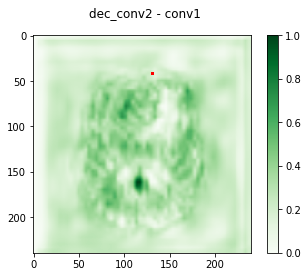
\includegraphics[width=\linewidth]{chapters/04_segmentation/images/grad_cam_24.png}
        \caption{First batch norm layer of the first encoder block}
    \end{subfigure}%
        \begin{subfigure}{.33\textwidth}
        \centering
        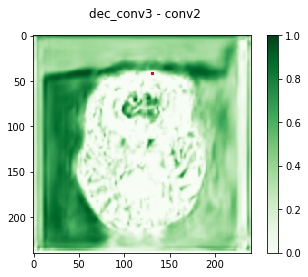
\includegraphics[width=\linewidth]{chapters/04_segmentation/images/grad_cam_29.png}
        \caption{First batch norm layer of the first encoder block}
    \end{subfigure}

    \begin{subfigure}{.33\textwidth}
        \centering
        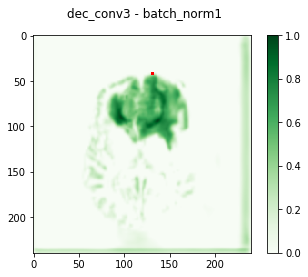
\includegraphics[width=\linewidth]{chapters/04_segmentation/images/grad_cam_30.png}
        \caption{First batch norm layer of the first encoder block}
    \end{subfigure}%
    \begin{subfigure}{.33\textwidth}
        \centering
        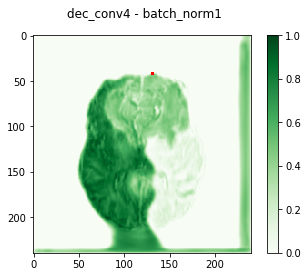
\includegraphics[width=\linewidth]{chapters/04_segmentation/images/grad_cam_34.png}
        \caption{First batch norm layer of the first encoder block}
    \end{subfigure}%
        \begin{subfigure}{.33\textwidth}
        \centering
        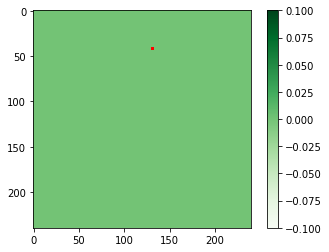
\includegraphics[width=\linewidth]{chapters/04_segmentation/images/grad_cam_36.png}
        \caption{Output convolutional layer}
    \end{subfigure}
    \caption{Explanation text}
\end{figure}

\subsection{Discussion}
TODO

\subsection{Conclusion}
TODO

Because of these results, we decided to not modify Grad-CAM to work on multiple pixels and move to other methods.